Thinking...
The user asks: "以下のの日本語文を英訳してください。ただしTeXのコードが挿入されているのでその部分はそのまま出力してください：" Then provides a LaTeX figure environment with Japanese caption "PubMedの収録論文数". So we need to translate the Japanese text, but keep the TeX code unchanged.

The Japanese text includes the caption: "PubMedの収録論文数". Possibly also the rest of the text "以下のの日本語文を英訳してください。ただしTeXのコードが挿入されているのでその部分はそのまま出力してください：" is instruction, not part of translation. Only the provided snippet should be output with translation for the Japanese parts, preserving TeX code.

Thus we need to output:

\begin{figure}[h]
\begin{center}
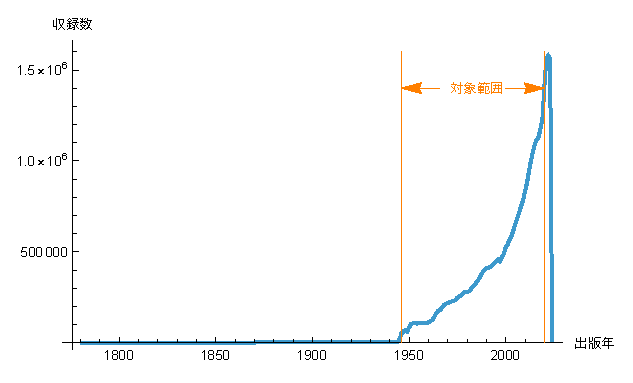
\includegraphics[width=76mm]{gr1.eps}
\caption{Number of articles indexed in PubMed}
\label{fig:gr1}
\end{center}
\end{figure}

Make sure to keep same line breaks. Possibly also translate any other Japanese like "PubMedの収録論文数". That's the only Japanese. So final answer is the LaTeX snippet with translated caption.
...done thinking.

\begin{figure}[h]
\begin{center}
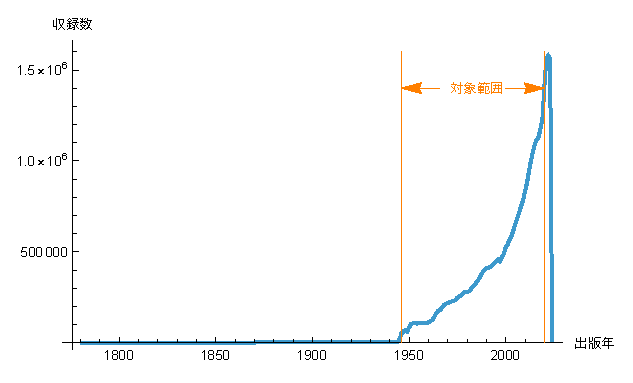
\includegraphics[width=76mm]{gr1.eps}
\caption{Number of articles indexed in PubMed}
\label{fig:gr1}
\end{center}
\end{figure}

